\documentclass[a4paper,openright,twoside,11pt]{report}
\usepackage[utf8]{inputenc}
\usepackage[english]{babel}

\usepackage[acronyms, nonumberlist]{glossaries}
\newacronym[plural={Json Web Tokens}]{jwt}{JWT}{Json Web Token}
\newacronym[plural={Application Programming Interfaces}]{api}{API}{Application Programming Interface}
\newacronym{rest}{REST}{Representational State Transfer}
\newacronym[plural={Data Access Layers}]{dal}{DAL}{Data Access Layer}
\newacronym[plural={Structured Query Languages}]{sql}{SQL}{Structured Query Language}
\newacronym[plural={Relational Database Management Systems}]{rdmbs}{RDMBS}{Relational Database Management System}
\newacronym[plural={User Interfaces}]{ui}{UI}{User Interface}
%{long}{jwt}{name={JWT},description={JSON Web Token}}
\usepackage{lipsum} % gerador de texto
\usepackage{graphicx}
\usepackage{url}

\usepackage{datetime}


\newdateformat{monthyeardate}{%
	\monthname[\THEMONTH], \THEYEAR}
\usepackage{ragged2e}
\usepackage[export]{adjustbox}
\usepackage{indentfirst}
\usepackage{xr}
\usepackage{hyperref}
%\bibliographystyle{plain}



% Definições das dimensões das páginas
\setlength{\textheight}{24.00cm}
\setlength{\textwidth}{15.50cm}
\setlength{\topmargin}{0.35cm}
\setlength{\headheight}{0cm}
\setlength{\headsep}{0cm}
\setlength{\oddsidemargin}{0.25cm}
\setlength{\evensidemargin}{0.25cm}

\makeglossaries
\usepackage[nottoc]{tocbibind}


% Página inicial (capa)
\title{
	\vspace{-50mm}
	\begin{minipage}[l]{\textwidth}
		\hspace{-20mm}\resizebox{75mm}{!}{
\includegraphics{./images/logoISEL.png}}\\
	\end{minipage}\\[20mm]
	{\bf ToDo - System for managing user's To Do list}
}

% Nome dos autores (um por linha)
\author{
	\begin{tabular}{ll}
		& Bernardo Rodrigues
\end{tabular}}

\date{
	\begin{tabular}{ll}
		{Supervisor:} & Nuno Leite \\
	\end{tabular}\\[10mm]
	% Deixar o indicador respetivo em função da versão do relatório.
	Report written for Project and Seminary\\
	from the Bachelor’s Degree in Computer Science and Computer Engineering\\[20mm]
	\monthyeardate\today}

\begin{document}
	\renewcommand{\bibname}{References}
	\renewcommand{\abstractname}{\vspace {-\baselineskip}}
	\thispagestyle{empty}
	\maketitle

	\baselineskip 18pt % line spacing: 12pt for single, 18pt for 1 1/2, and 24pt for double spacing
	
	\newpage
	\pagenumbering{roman}
	% Fim da contracapa

	
	% Página com identificação completa (número e nome) e assinaturas do(s) estudante(s) e do(s) orientador(es)
	

	
	
	% Página de resumo em Português
	\cleardoublepage

	
	\tableofcontents

	
	\printglossary[type=\acronymtype, title=List of Acronyms]

	
	\listoffigures
	
	%web push protocol https://tools.ietf.org/html/draft-ietf-webpush-protocol-12


	\pagenumbering{arabic}
	\setcounter{page}{1}
	\chapter{Introduction}

In today’s fast and complex world people try to schedule days or weeks. People create small
reminders, either electronically or physically, to do something, whatever that may be. Those
little notes we give to ourselves, those ”to-do’s” are often forgotten and not fully fulfilled.
There exists software applications in the market that partially accomplishes this goal. They will often remind the user of the task that needs to be done only using the time frame the user gave. This creates a problem where the individual makes a reminder,
does not do it and the application will not keep notifying the user.\\
As such the proposed solution will attempt to mend that by creating an environment where a reminder is easily
created but hardly forgotten or skipped over. The solution consists of a web application divided into three different components, a front-end web app, a back-end web \gls{api} and a database. This application will allow the users to create
an account and then make reminders. The users will be notified by the application until they mark said reminder as done.\\
The notification is a necessity to ensure the user fulfills the reminder. Since the user will be notified until the reminder is marked as "done" the person will be reminded every day until the completion of the task.

For this purpose a set of mandatory requirements was outlined:
\begin{itemize}
	\item Account creation, login, logout and account deletion;
	\item Reminder creation, update and deletion;
	\item Notifications;
\end{itemize}

Some optional requirements were also outline to enrich the application:
\begin{itemize}
	\item Translations
	\item Priority notifications
\end{itemize}

This report will outline the process of the application development, the choices made and the work
that remains to be done.
	
	\chapter{Architecture}

	%https://martinfowler.com/articles/microservices.html
	%
	
	
	
	The architecture for the API was thoroughly researched and studied. At first this project was gonna use a monolithic architecture \cite{monolith} where the whole API would be implement on a single server as seen in the image below.
	%TODO add image of monolith arch
	
	This was later changed due to the fact that it wasn't as easily scalable \cite{scale}. After this it was decided that the API would be implemented using a \textit{microservice}\cite{microservice} architecture. This allows for a more select scalability. When needed, more instances of the same services can be launched and improve overall performance.
	
	There will be different services:
	\begin{enumerate}
		\item User
		\item To-do
		\item Task
	\end{enumerate}

	%TODO add image here add image of micro-service arch
	
	There was also the idea of combining both the monolithic and micro-service architecture in a mixture of both patterns. This idea was later scrapped and the micro-service system was then chosen.
	
	%TODO add image of monolith - microservice arch
	
	Each of these services are independent from one another and self sufficient, each with it's own responsibilities. 
	
	%https://tools.ietf.org/html/rfc7519
	%https://www.rfc-editor.org/rfc/pdfrfc/rfc7519.txt.pdf
	
	% https://www.cs.cmu.edu/afs/cs/project/vit/ftp/pdf/intro_softarch.pdf
	
	\section{User}
	The user micro-service will have the operations needed for an user to utilize the application. These operations consist of the sign up, login, logout and, delete.
	The micro-service will use \gls{jwt} \cite{jwt} as a way to make sure the users only access their information.
	The service is split into two different areas, the repository\cite{repositorypattern} that accesses the database and ,the routing.
	
	\section{To-do}
	The to-do micro-service handles all the operations necessary to manage the to-do's. These operations embedded in this service are to-do creation, deletion and update.
	This micro-service will interact with the user service to validate and extract the \gls{jwt} information.
	
	\section{Task}
	The task micro-service has three main objectives. It offers a way to subscribe and unsubscribe users to receive notifications as well as checking the database periodically to ensure the notifications are sent to the subscribed users. The notifications will be sent according to the push protocol\cite{pushprotocol}.
	 
	
	\chapter{Database and Data Modeling}

	The database model is described, in this chapter. It's a fairly simple model although additions can be made to augment and improve the application's features.

	\begin{figure}[h!]
		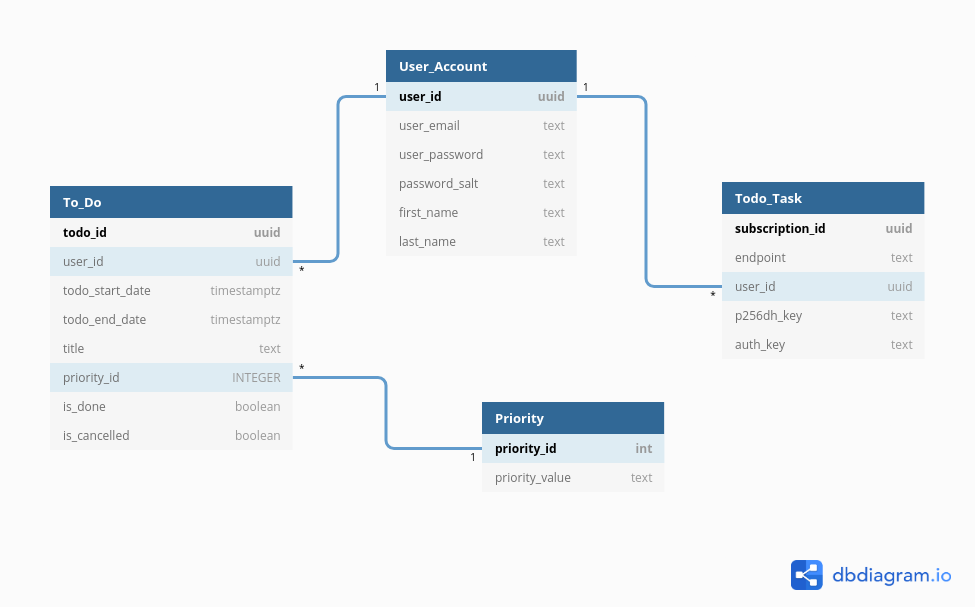
\includegraphics[width=17cm,scale=0.6]{./images/data_model_2do}
		\caption{Data Model}
	\end{figure}

	A user can have multiple to-do's and subscriptions (tasks). The need for multiple subscriptions stems from the fact that the user can have multiple instances of the application running in different desktops.\\
	There also is a priority system which hasn't yet been implemented. In the future each to-do will have a priority with a specific value and this value will be used to calculate how many times the user will be notified.
	
	
	\chapter{API}
	
	%add api doc
	%communication flow in the api
	%protocols
	%security
	%packages used
	%etc
	
	\chapter{Conclusions}

	Creating a reminder system with specific granularity and prioritization has it's difficulties. Even though the \gls{api} was implement and is functioning the challenges of the development were more than previously analyzed. The implementation of the notification system was arduous and the micro-service architecture, even though useful and extremely scalable, proved to be challenging. The application itself has a lot of potential future work since it can be improved and is more of a proof of concept.\\
	The front-end application can be improved but as previously mentioned it was a proof of concept.
	Future improvements to the application would make it more user friendly and usable.
	
	\bibliographystyle{unsrt}
	\bibliography{rp}
	
\end{document}